\documentclass[twocolumn]{article}  
\usepackage[top = 1.5cm, bottom = 1.5cm, left = 1.0cm, right = 1.0cm]{geometry}  
\usepackage{graphicx}
\usepackage{amsmath}  
\usepackage[inline]{enumitem}
\setlength{\columnseprule}{0.4pt}
\setlength{\columnsep}{3em}
\makeatletter
% This command ignores the optional argument for itemize and enumerate lists
\newcommand{\inlineitem}[1][]{%
\ifnum\enit@type=\tw@
    {\descriptionlabel{#1}}
  \hspace{\labelsep}%
\else
  \ifnum\enit@type=\z@
       \refstepcounter{\@listctr}\fi
    \quad\@itemlabel\hspace{\labelsep}%
\fi}
\makeatother

\title{DL Assignment-01}
\date{}
\author{Rohan Anil Muskawad\\2020A8PS1798P}
\begin{document}  
\maketitle

\section{[Page 83 -to- 85]}

\begin{enumerate}
        
        \item Group which contains the maximum number of student is
            \begin{enumerate}
                \item 130-140 \inlineitem 140-150
                \item 150-160 \inlineitem 160-170
                
            \end{enumerate}
                \textbf{Direction(2):}Study the histogram of weight distribution of different men and answer question based on it
            \begin{flushright}
                \textbf{[SSC CGL 2013]}
            \end{flushright}

            \begin{center}
                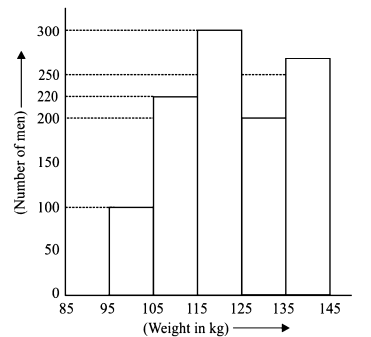
\includegraphics[scale=0.7]{pic1.png}
            \end{center}
            
        \item Average number of men per interval who participated in the survey is
            \begin{enumerate}
                \item 180
                \inlineitem 194
                \item 200
                \inlineitem 214
            \end{enumerate}

            \textbf{Direction(3-4):}The histogram shows the marks of 50 students in an examination. Examine the diagram and answer the question \hfill\textbf{[SSC MTF 2013]}
            
            \begin{center}
                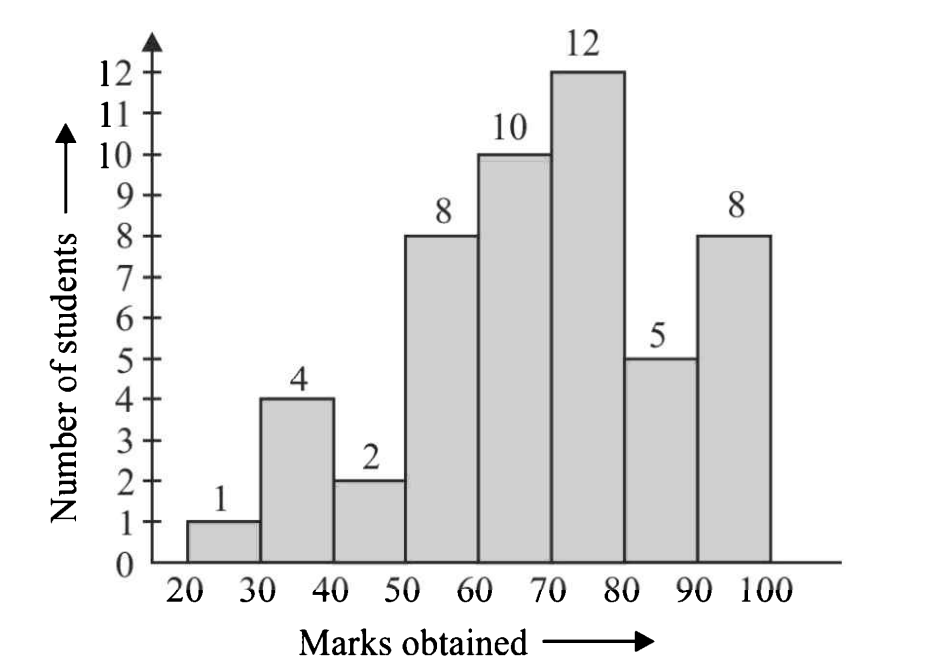
\includegraphics[scale=0.8]{pic2.png}
            \end{center}

        \item How many students obtained more than 39 but below 60?
            \begin{enumerate}
                \item 6
                \inlineitem 8
                \item 10
                \inlineitem 12
            \end{enumerate}

        \item What percent of students did obtain marks above 60\%
        \begin{enumerate}
            \item 60\%
            \inlineitem 70\%
            \item 75\%
            \inlineitem 80\%
        \end{enumerate}
        \textbf{Direction(5-6):}Study the graphs carefully and answer the qeustion \hfill\textbf{[SSC CGL 2013]}
        \begin{center}
            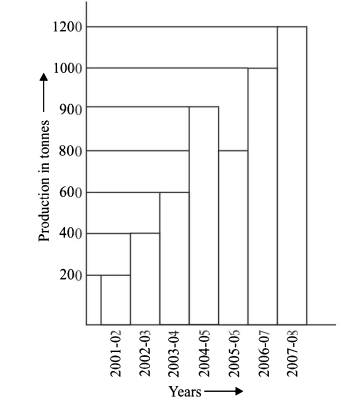
\includegraphics[scale=0.8]{pic3.png}
        \end{center}
        \item The production in 2006-07 in comparison to the production in 2002-03 increased by
            \begin{enumerate}
                \item 110\%
                \inlineitem 120\%
                \item 125\%
                \inlineitem 150\%
            \end{enumerate}
\end{enumerate}


\end{document}
